\subsection{Assessment of Final Design}
Upon evaluation of the project requirements, needs, and constraints identified, it can overall be stated that the design project was a success and completed to the satisfaction of the stakeholders. The primary deliverable of the project was to develop a process for predicting the lag temperature of the metal cylinder using a machine learning algorithm and to use the information to estimate the soak time. We were able to accomplish our objective using Python along with LSTM neural networks and Random Forests for our machine learning algorithms. A comparison of the effectiveness of the LSTM method and Random Forests method can be seen in Figure \ref{fig:real_data_error_rs_lstm1} and Figure \ref{fig:real_data_error_rs_lstm2}. It can be seen from the graphs that the LSTM method is overall more reliable and superior compared to the Random Forests method, as the percent error is generally smaller, more consistent, and less sporadic. The error patterns observed for LSTM represent mostly an offset whereas the patterns observed for Random Forests are more random. Furthermore, the LSTM method is more effective for determining soak time as the prediction by the end of the cycle is more accurate. The estimation of the soak time was implemented into our Python scripts. The system designed for this project establishes an Industry 4.0 framework that can be further expanded upon, and overall the final design is an effective proof of concept for demonstrating the feasibility of this system for composites manufacturing. A practical solution for finding the soak time was implemented in a testing process where it is otherwise unknown.\\\\
In consideration of our other project needs and constraints, we were able to improve and further optimize the data collection process. Better thermistors were purchased and their optimal placement was determined through testing. An ADC was also purchased and these changes allowed us to improve accuracy in our sensor readings and confirm that our results were consistent. The signal-to-noise ratio was taken into consideration as we ran the collected data through filters in order to boost the signal-to-noise ratio. The budget constraint was not a concern, as roughly half of the budget was used throughout the entire project. Safety precautions were always taken while testing in the lab and no danger was ever present. \\\\
One disappointment in our project is that only a small sample of valid data was collected and used for developing the machine learning processes. The small amount of data retrieved was due to limited access to the Composites lab following the COVID-19 outbreak. With minimal data collected, the integration of cloud storage through IBM Cloud was invalidated as it would not be useful for a small data set. Ultimately, most of the requirements, needs, and constraints established by the stakeholders were successfully accommodated and fulfilled. 

\begin{figure}[ht]
    \begin{subfigure}{.5\linewidth}.
        \centering
    	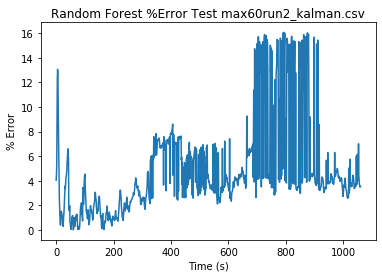
\includegraphics[width=\linewidth]{other/RF_error_real2.png}
    \end{subfigure}
    \begin{subfigure}{.5\linewidth}
    	\centering
    	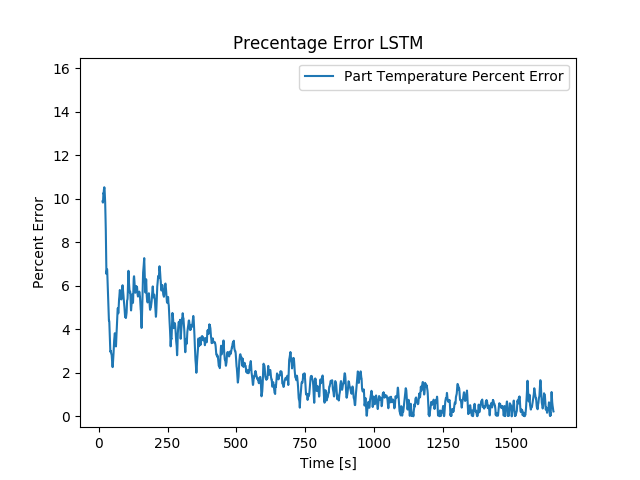
\includegraphics[width=1.01\linewidth]{lstm/run2_rescale.png}
    	\vspace{.05pt}
    \end{subfigure}
    \caption{Real Data Percent Error Comparison}
    \label{fig:real_data_error_rs_lstm1}
\end{figure}
\begin{figure}[ht]
    \begin{subfigure}{.5\linewidth}.
        \centering
    	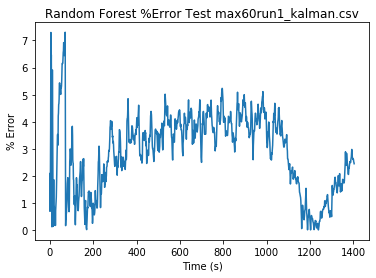
\includegraphics[width=\linewidth]{other/RF_error_real.png}
    \end{subfigure}
    \begin{subfigure}{.5\linewidth}
    	\centering
    	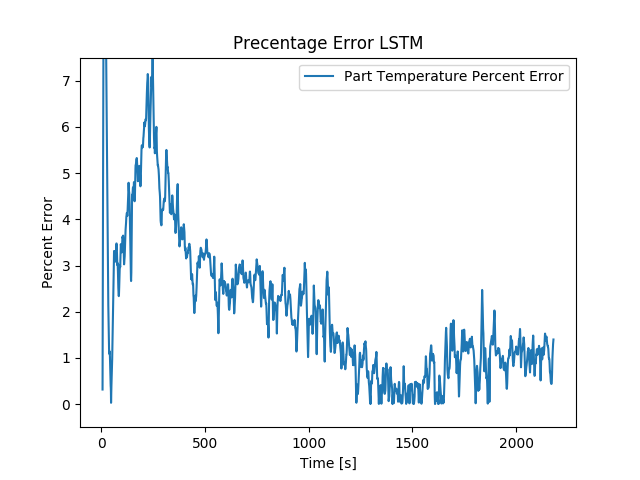
\includegraphics[width=1.01\linewidth]{lstm/run1_rescale.png}
    	\vspace{.05pt}
    \end{subfigure}
    \caption{Real Data Percent Error Comparison}
    \label{fig:real_data_error_rs_lstm2}
\end{figure}
\newpage
\subsection{Coronavirus Restrictions}
Due to closure of non-essential laboratories at UBCO in response to COVID-19 as of March 17, 2020, there were a number of topics we were unable cover or implement. In particular, we were unable to gather more reliable data using our redesigned  Raspberry Pi based data acquisition unit. With more data, we would be able to more thoroughly validate our machine learning models. In addition, while the code to predict internal temperature in real-time exists, as we were unable to gain access to the laboratory, we were unable to implement or test this feature with the heat chamber.

\subsection{Recommendations for Future Work}
There are a number of recommendations that can be made for further progressing this project. Some suggestions include: further testing, improving the simulations for generated data, data assimilation, and transfer learning. 
\subsubsection{Further Testing}
One avenue for future work is expanding upon the machine learning process through further testing. This includes gathering additional data for the aluminum cylinder used in this project as well as a comparable volume of data for other parts consisting of different materials and shapes to be used for further training the machine learning models. As it is eventually the goal to implement this type of system for determining the soak time for composite materials, it is necessary to incrementally train and update the machine learning models developed for this project to accommodate other parts and materials before being accessible to composites. \newline
\begin{wrapfigure}{r}{0.5\textwidth}
  \vspace{-50pt}
  \begin{center}
    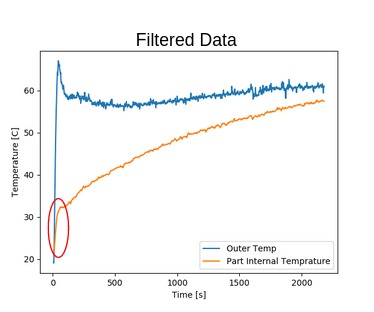
\includegraphics[width=0.50\textwidth, height = 80mm]{other/filt_data_circle.png}
  \end{center}
  \vspace{-20pt}
  \caption{Filtered Data showing }
  \label{fig:filtered_data_circle}
  \vspace{-20pt}
\end{wrapfigure}
Another test we wanted to perform but were not able to due to separation of the logger and PI controller was to extract the duty cycle of the PI controller over the run. As seen in Figure \ref{fig:filtered_data_circle} to the right and circled in red, there is a steep rising curve initially for the part temperature which is likely due to an increased amount of heat transferred through radiation because the infrared lamp was on for high duty cycles in our collected data, and without extracting the duty cycle we could not use that information at the initial point in time. It is expected that with this additional information the machine learning algorithm would have an easier time adjusting for the offset that the part temperature is at throughout the run.  \\

\subsubsection{Improving Simulations}
There are some limitations in the simulations performed for this project, and further improvements in the simulation parameters would aid in validation of the machine learning models and the data collected. In the MATLAB simulations performed, a two-dimensional rectangle was modeled to approximate the three-dimensional cylinder used in the project. While this was a simpler process, more accurate and reliable data could be generated by importing an identical 3D mesh of the cylinder for the simulation runs.  \\\\
Another adjustment that could be made to the simulations is to account for more parameters. For simplicity, the model used for the simulations referenced in this report only account for conductive heat transfer, but a more thorough model would also account for convective heat transfer and radiation. The thorough model is more useful as it provides a more accurate and practical view of the heating system and its properties.
\subsubsection{Data Assimilation}
Another possible improvement for this project is data assimilation which is the use of computer generated data such as a simulation combined with real world data to create synthetic data which is assimilated with the real data to train a neural network. As we have both of these components, further testing could be implemented. It was found that the simulation needed to be tweaked further to attain data that improved the prediction ability. A small amount of testing was conducted in this area on the LSTM model but it was found that it did not improve the prediction ability on real data. It may have only decreased over-fitting of the model. It is challenging to come to a definite conclusion, especially since the simulated data vastly outnumbers the real data. The most interesting result from data assimilation would be to decrease the number of real runs that need to be conducted therefore this would be an area for further research.
\subsubsection{Transfer Learning}
Lastly, a worthwhile concept to look into is Transfer Learning. Transfer Learning is a domain of machine learning which uses the training data or model from one problem and adapts it towards a new but related problem. As we saw some cases of over-fitting during our testing, transfer learning could possibly used as an option to counteract over-fitting and improve generalization performance. In particular, Transfer Learning could work well in cases where we have a limited amount of training data for a certain target scenario (e.g. new material, different object geometry) but have related data from previous experiments or other data sets. Some interesting Transfer Learning methods to look into include \cite{daume07easyadapt}, and \cite{DBLP:journals/corr/SunFS15}. Both of these Transfer Learning methods have good performance and are simple to implement and require less than 10 lines of code. 